\section{Communication à l'aide de signaux}
	Afin de permettre aux threads d'interagir entre eux, nous
        avons ajouté un système de signaux.  Ces signaux se
        représentent sous la forme d'entiers positifs qui sont stockés
        dans une liste dans la structure du thread. Ils peuvent être
        envoyés grâce à la fonction $thread\_kill$ prenant un
        paramètre un $thread\_t$ représentant le thread auquel envoyer
        le signal et un $int$ représentant le signal à envoyer.\\
	
	Ces signaux sont traités lors du passage au sein d'une des
        fonctions de la librairie, lors de son retour en exécution,
        l'ordonnanceur va effectuer les traitements de tous les
        signaux dans l'ordre de leur réception pendant que le thread
        était dans la file d'attente. Il y a pour le moment 6 signaux
        définis, un pour faire s'interrompre le thread, un autre, pour
        lui faire passer la main et les 4 autres sont des signaux
        personnalisables.\\
	
	Nous avons de plus permis de personnaliser le traitement de
        certains signaux, à l'aide d'une table de signaux propre à
        chaque thread. Cette table est renseignée à l'aide de la
        fonction $thread\_signal$ prenant en paramètre le thread à
        modifier, le signal auquel attribuer la fonction et un
        pointeur de fonction de signature $void(*func)(int)$ qui sera
        la fonction appelée lorsque le thread recevra le signal.\\
	
	Le programme $test\_signal$ teste l'implémentation de ces
        signaux. Il crée un thread qui fait deux boucles while, la
        première laissant la main à chaque tour et s'arrêtant
        lorsqu'il reçoit le signal $SIG\_USR1$, la seconde ne faisant
        rien. Ce thread reçoit à la suite un signal $SIG\_USR1$ et
        $SIG\_KILL$, on remarque dans l'exécution que le signal
        $SIG\_KILL$ est traité avant la sortie de la première boucle
        (absence de l'affichage "out of the loop").\\
	
	
\begin{figure}[h]
  \begin{minipage}[c]{.45\linewidth}
    \begin{center}
      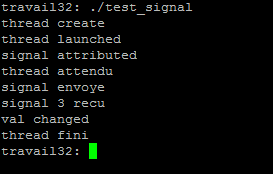
\includegraphics[height=2cm]{test_signal.png}
      \caption{Ex\'ecution de test signal}
      \label{test signal}
    \end{center}
  \end{minipage}
\end{figure}


	Nous avons par la suite implémenté la possibilité aux threads
        d'envoyer des signaux à l'ordonnanceur concernant certains
        threads à l'aide de la fonction $thread\_signal$ sauf que les
        signaux envoyés sont alors des entiers négatifs. Ainsi nous
        avons défini deux signaux ordonnanceurs, un pour demander la
        suspension de l'exécution d'un thread actuellement dans un
        état exécutable, et un autre pour le remettre dans la liste
        des threads exécutables.\\
	
	Cette fonctionnalité est testée par le programme $test\_stop$
        qui exécute deux threads parallèlement affichant les nombres
        de 1 à 10 et laissant la main entre chaque affichage. Une fois
        la première moitié faite, le premier thread va envoyer à
        l'ordonnanceur de retirer le deuxième thread à l'aide du
        signal $SIG\_STOP$, représenté par la ligne "Attaque seau de
        colle!!" lors de l'exécution. On voit alors que le premier
        thread finit de compter jusqu'à 10, une fois qu'il a fini de
        compter, il envoie le signal $SIG\_WAKE$ pour réveiller le
        deuxième thread. Or remarque que le deuxième thread finit
        alors de compter.\\

\begin{figure}[h]
  \begin{minipage}[c]{.45\linewidth}
    \begin{center}
      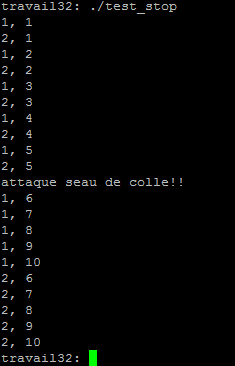
\includegraphics[]{test_stop.png}
      \caption{Ex\'ecution de test stop}
      \label{test stop}
    \end{center}
  \end{minipage}
\end{figure}
